\documentclass{tufte-handout}
% Settings
 \date{Jul 12, 2024} % without \date command, current date is supplied
 %\geometry{showframe} % display margins for debugging page layout
 % Load the packages
 \usepackage{graphicx} % allow embedded images
   \setkeys{Gin}{width=\linewidth,totalheight=\textheight,keepaspectratio}
   \graphicspath{{graphics/}} % set of paths to search for images
 \usepackage{amsmath}  % extended mathematics
 \usepackage{blindtext}
 \usepackage{units}    % non-stacked fractions and better unit spacing
 \usepackage{multicol} % multiple column layout facilities
 \usepackage{lipsum}   % filler text
 \usepackage{booktabs} % For professional looking tables
 \usepackage{fancyvrb} % extended verbatim environments
   \fvset{fontsize=\normalsize}  % default font size for fancy-verbatim environments
 \usepackage{glossaries}
   \setacronymstyle{long-short}
 \usepackage{verbatim}

 % Standardize command font styles and environments
 \newcommand{\doccmd}[1]{\texttt{\textbackslash#1}}% command name -- adds backslash automatically
 \newcommand{\docopt}[1]{\ensuremath{\langle}\textrm{\textit{#1}}\ensuremath{\rangle}}% optional command argument
 \newcommand{\docarg}[1]{\textrm{\textit{#1}}}% (required) command argument
 \newcommand{\docenv}[1]{\textsf{#1}}% environment name
 \newcommand{\docpkg}[1]{\texttt{#1}}% package name
 \newcommand{\doccls}[1]{\texttt{#1}}% document class name
 \newcommand{\docclsopt}[1]{\texttt{#1}}% document class option name
 \newenvironment{docspec}{\begin{quote}\noindent}{\end{quote}}% command specification environment

%\makeglossaries % Generate the glossary
 \loadglsentries{defns}
% To solve the additional V padding made by \newthought
 \makeatletter
 \def\tuftebreak{%
  \if@nobreak\else
    \par
    \ifdim\lastskip<\tufteskipamount
      \removelastskip \penalty -100
      \tufteskip
    \fi
  \fi
 }
 \makeatother

\title{Micro Gravity and \gls{aqe}}
\author{\small Laurent Lathieyre | llathieyre@gmail.com | 425-229-7272}
\begin{document}
\maketitle % this prints the handout title, author, and date
\small Last Update: July 12, 2024

%\begin{figure}
%    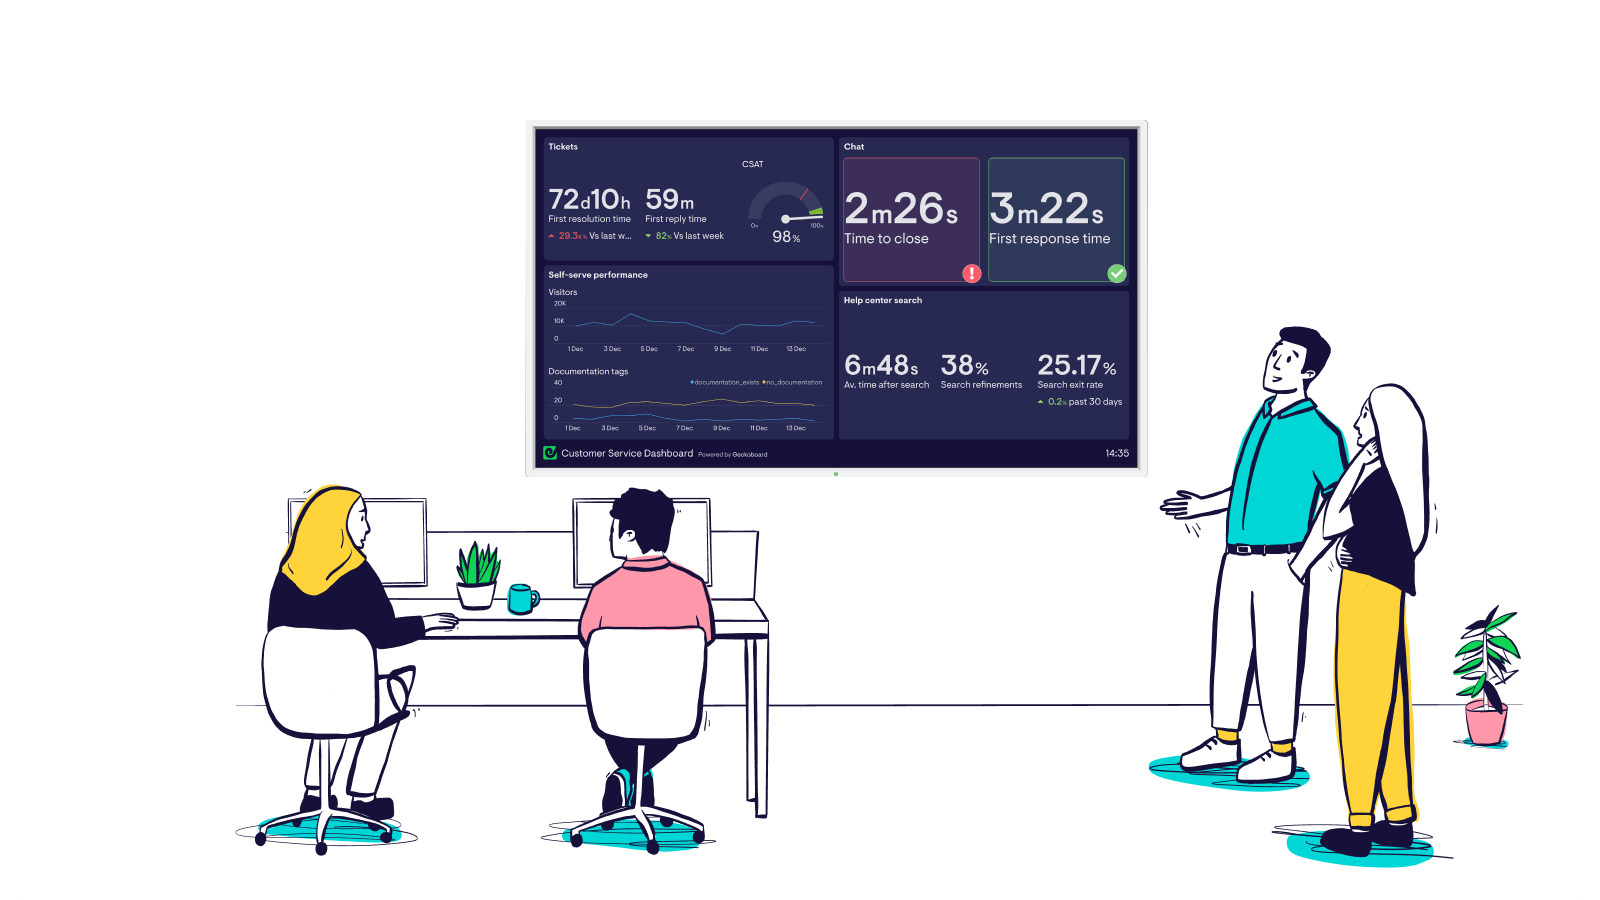
\includegraphics{share-tv.png}
%\end{figure}

\section{TL;DR}\label{sec:tldr}
\newthought{\gls{genai} is a new technology} that can help us create new user interfaces. It can help us design better user experiences, faster and more efficiently. It can also help us create new types of user interfaces that were not possible before. 

I believe \gls{genai} is already having a tremendous impact on the way users consume technology. For example, the natural language conversational interaction mode could be a \emph{game changer} for SaaS ISVs.\sidenote[][-20pt]{\textit{"I don't need your SaaS! Just give me acces to this AI thing!"} is often times the reaction I got from people I was demoing to the new \gls{genai} companion to a Contract Lifecycle Management SaaS product directly integrated within Microsoft Word. This also demonstrates the importance of meeting the end-user whithin -- or close to -- the tools of their daily workflow.}

This document presents why I believe Slack could be the best conduit for us to future proof our competitiveness.\cite{pottsMaterialsScienceMicrogravity2023}

\section{What is \gls{aqe}?}\label{sec:what-is-azure-quantum-elements}
\newthought{\gls{aqe} is a cloud-based service} provided by Microsoft through Azure Quantum, designed to accelerate scientific discovery in the fields of chemistry and materials science. It integrates high-performance computing (HPC), artificial intelligence (AI), and quantum computing to enhance research and development productivity. Here are the key features and capabilities of \gls{aqe}:

\subsection{Key Features}\label{sec:key-features}
\paragraph{\gls{hpc}}\label{sec:hpc} \gls{aqe} leverages Azure's HPC clusters to scale simulation workflows, enabling researchers to perform complex calculations more efficiently.
\paragraph{AI-Accelerated Computing}\label{sec:ai-Accelerated} The service incorporates AI tools to augment reasoning and automate workflows, significantly reducing the time and effort required for scientific research. For example, the Generative Chemistry feature uses generative AI to simplify the discovery and design of novel molecules.
\paragraph{Quantum Computing Integration}\label{sec:quantum-computing-integration} \gls{aqe} provides tools to experiment with existing quantum hardware and prepares users for future quantum supercomputers. This integration allows for the simulation of molecular interactions at the quantum level, which classical computers cannot achieve.
\paragraph{Accelerated Density Functional Theory (DFT)}\label{sec:dft} The Accelerated DFT feature, available in private preview, can determine the quantum-mechanical properties of molecules with thousands of atoms in hours, offering a significant speed increase compared to traditional methods.
\paragraph{Natural Language Interface}\label{sec:natural-language-interface} The service includes a natural language interface, Copilot for Azure Quantum, which allows researchers to generate code, query and visualize data, and initiate simulations using conversational interactions. This feature makes advanced computational tools accessible to both experts and non-experts.

\subsection{Applications and Impacts}\label{sec:applicationss-and-impact}
\paragraph{Chemical and Materials Science}\label{sec:chemical-and-materials-science}
\gls{aqe} is designed to tackle some of the most complex problems in chemistry and materials science, such as developing new materials, drugs, and more efficient batteries. It aims to compress centuries of scientific progress into decades by providing powerful computational tools.
\paragraph{Sustainability and Innovation}\label{sec:sustainability-and-innovation}
The platform has been used in various industries to achieve breakthroughs that contribute to sustainability, such as improving battery technology and developing new pharmaceutical compounds. Companies like BASF and Johnson Matthey have adopted \gls{aqe} to enhance their research capabilities.
\paragraph{Future Prospects}\label{sec:future-prospects}
Microsoft plans to introduce advanced quantum computing capabilities, including a quantum supercomputer, which will further transform research and innovation across multiple industries. These advancements are expected to solve global scientific challenges by providing unprecedented computational power.
\paragraph{}\label{sec:summary}
In summary, \gls{aqe} is a comprehensive platform that combines HPC, AI, and quantum computing to revolutionize scientific research in chemistry and materials science, making complex simulations faster and more accessible.









\section{Rationale}\label{sec:Rationale}
\paragraph{The Most Valuable Real Estate}\label{sec:real-estate} Except for  email, where professionals spend close to 3~hours per day~\cite[+5pt]{mattplummerHowSpendWay2019}, only \emph{Communication and Collaboration software} such as Teams and Slack come close second. Which makes Slack a great place to start as it is a platform that is already used by many companies and has a large user base. 
It is also a platform that is already integrated with many other tools and services, which makes it easier to build on top of.

\paragraph{Multi Clouds and Innovation Beachhead}\label{sec:multi-clouds} Customers with 4+ Salesforce Clouds represent $20\%$ of total customers, driving $\approx 85\%$ of the total ARR. The average ARR per customer vs. single Salesforce Cloud customer increases drastically with the number of additional Clouds, along with a decrease in the attrition rate. \par
Slack can not only be the foundational cloud that connects all the Clouds, but also the most legitimate place to harbor new innovative ways of interactions, and new user experiences.
\begin{marginfigure}[-150pt]
  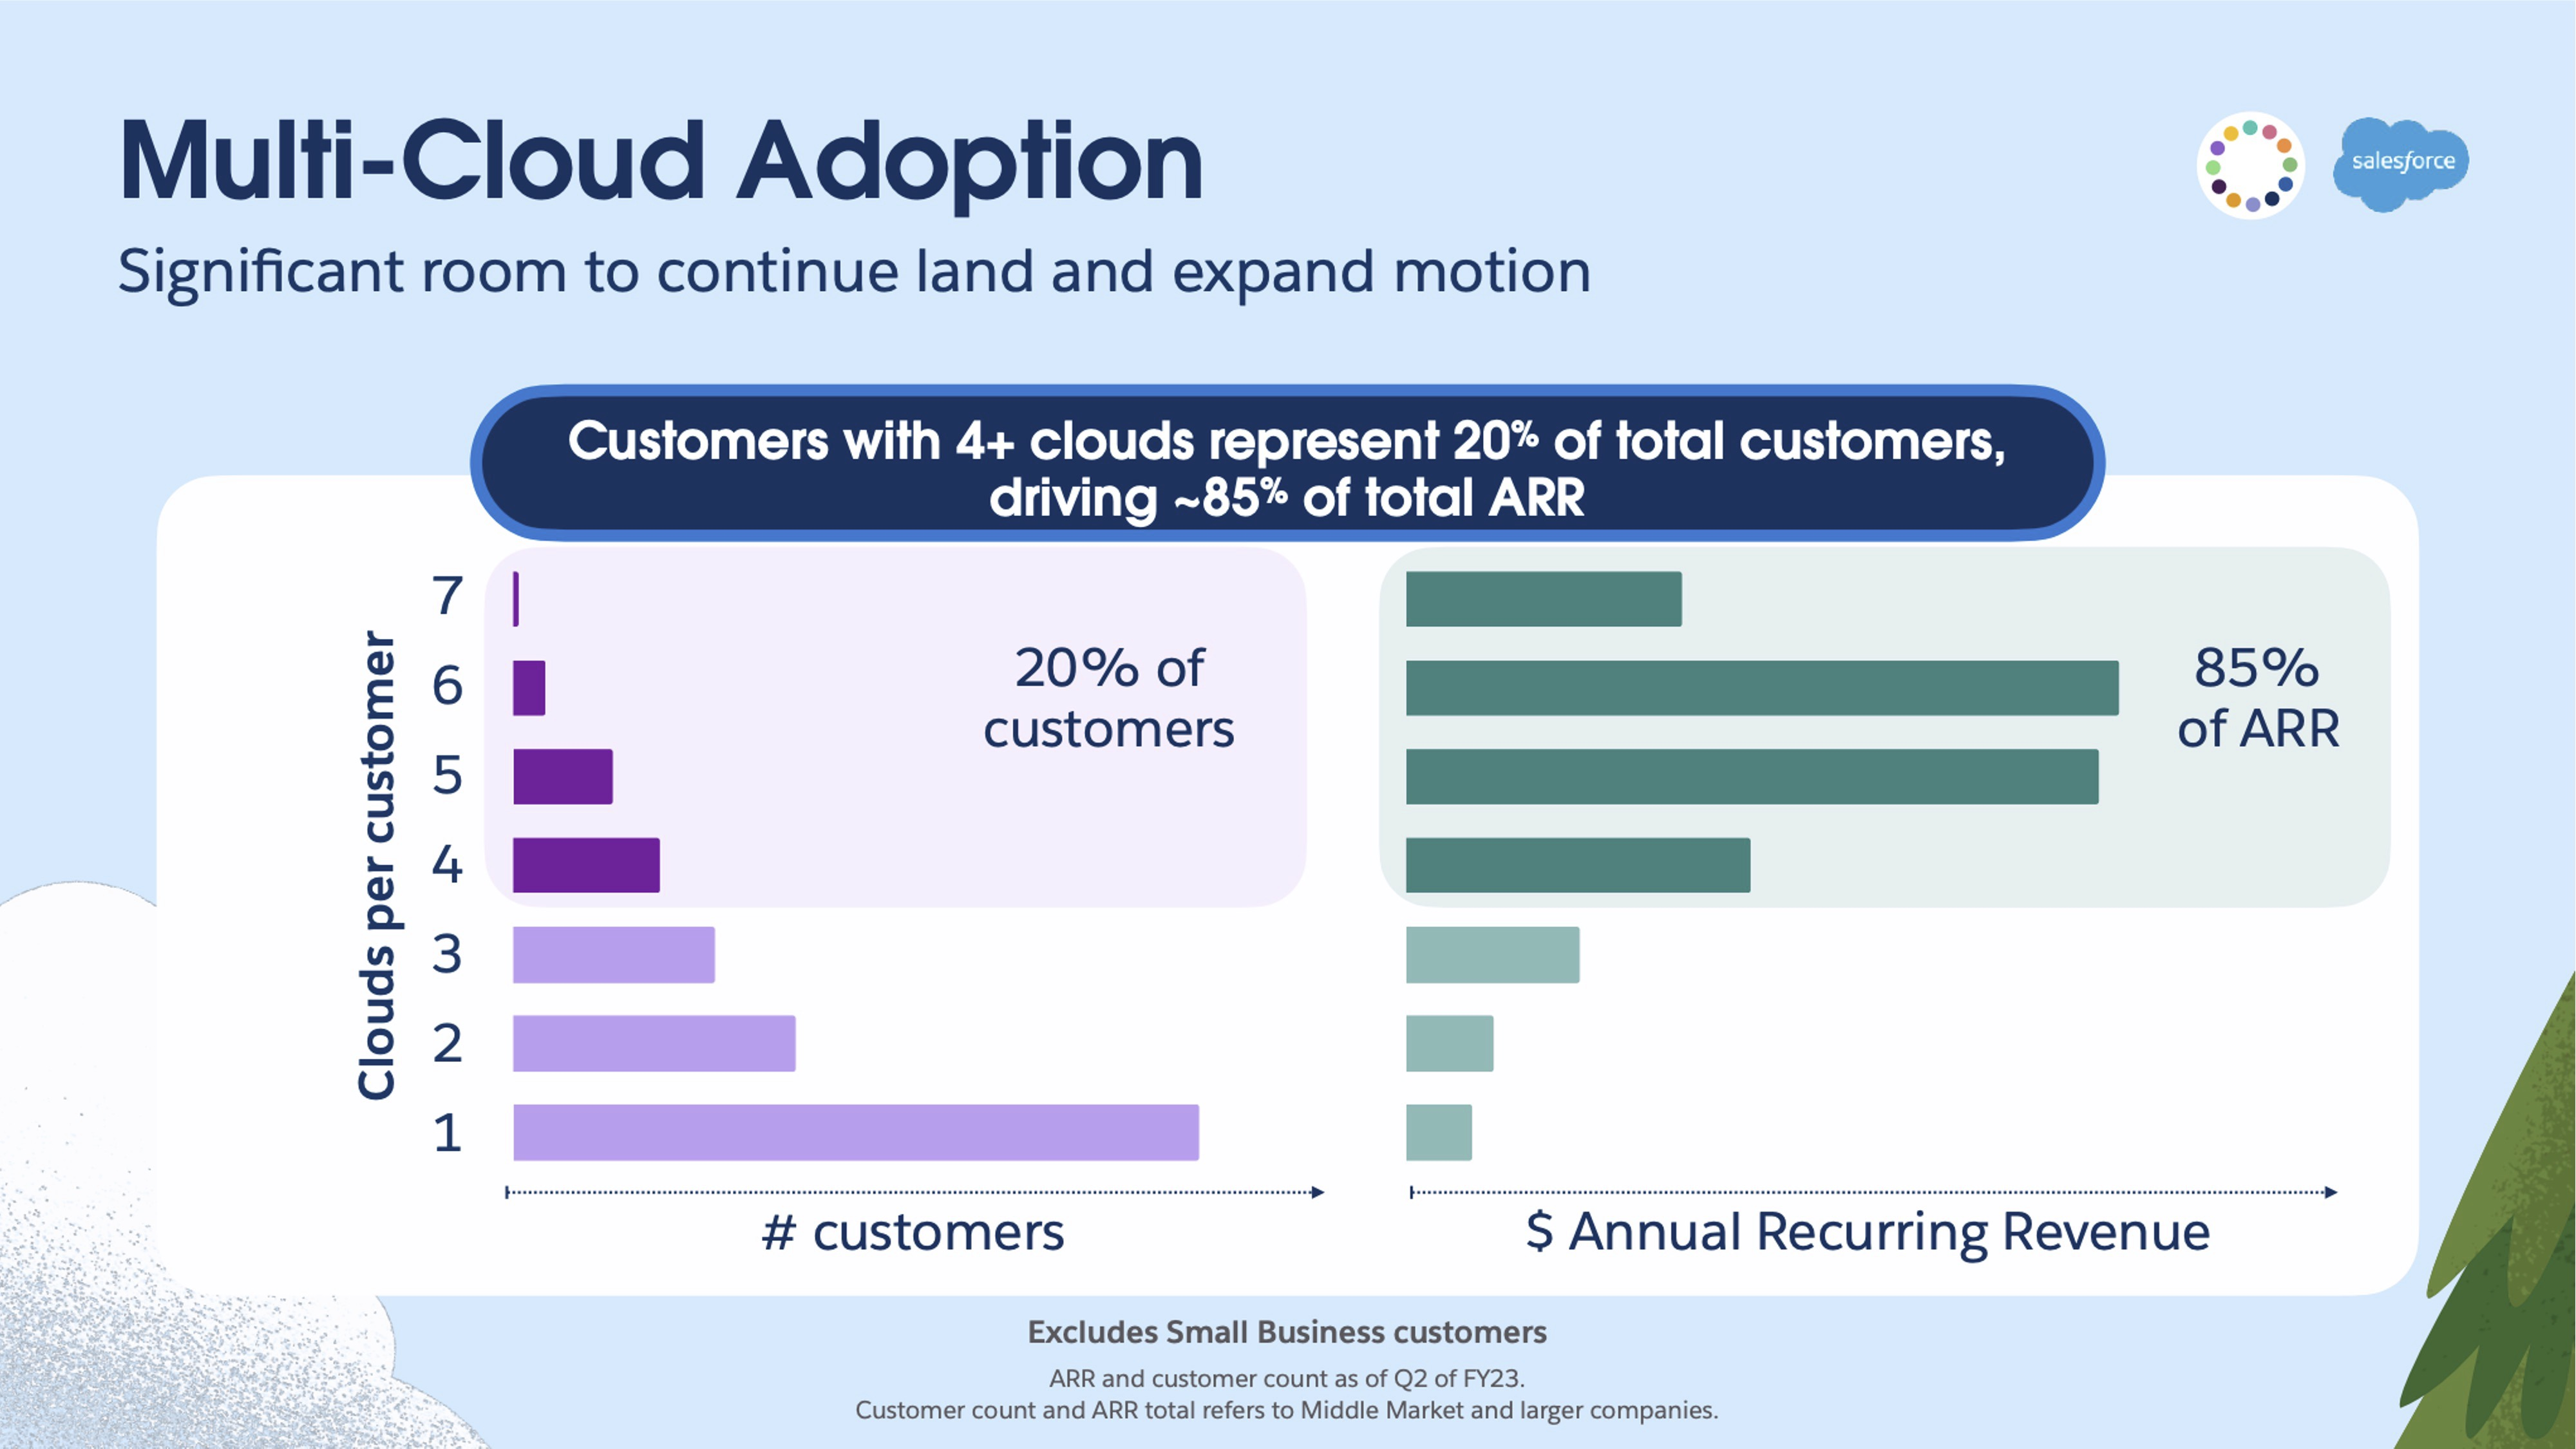
\includegraphics{salesforce-22}
  \caption{Multi Cloud Adoption}
\end{marginfigure}
 \begin{marginfigure}[-40pt]
  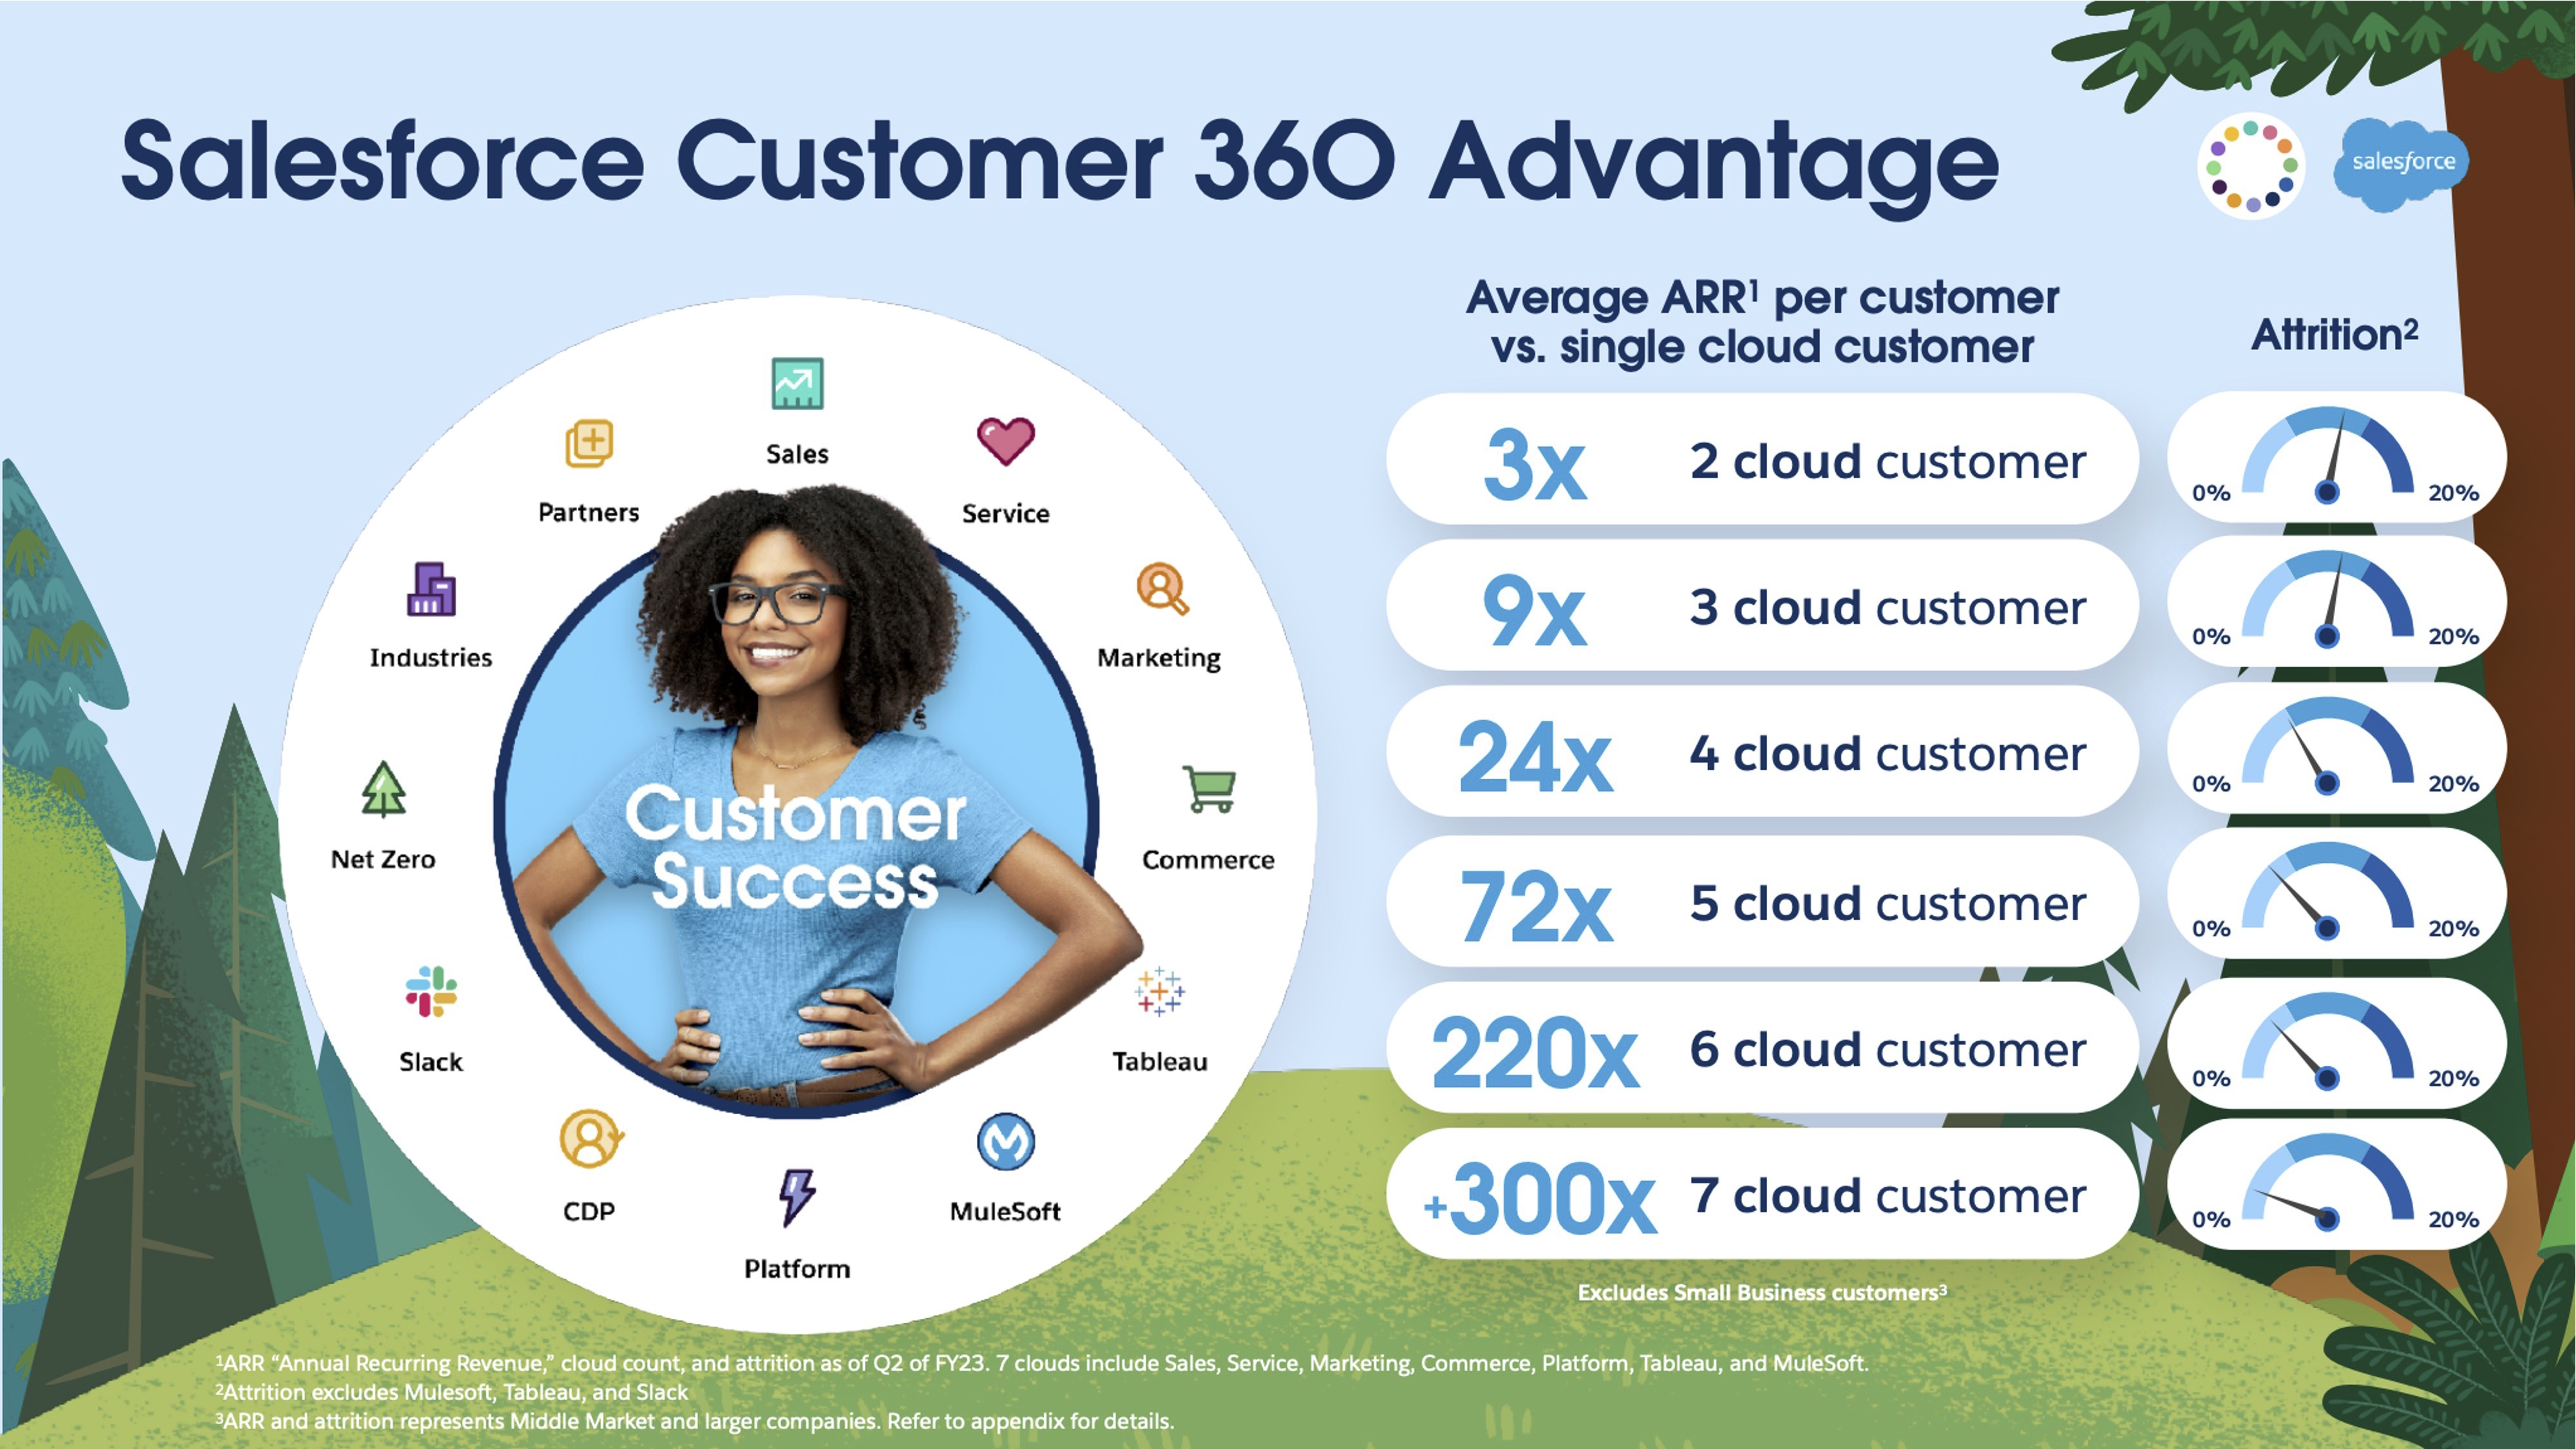
\includegraphics{salesforce-23}
  \caption{Single v. Multi Cloud ARR}
\end{marginfigure}
For example:
\begin{itemize}
  \item Use agentic AI for new types of collaboration and automation (e.g. \emph{group discussion} in a brainstorming channel with specialized AI Agents; Agent powered by a Large Action Model that can carry out  action plans on your behalf).
  \item Cover the \emph{last yard} of a Field Service worker by providing a hands-free speech-to-speech interface to Service Cloud.\sidenote{The open source project OpenInterpreter.com gives a glimpse of what could be done (speech interface, Large Action Models, LLM as the new Operating System). See video: \url{https://x.com/OpenInterpreter/status/1770821439458840846}}
\end{itemize}

\paragraph{Competition and Market Segments}\label{sec:competition-market-segments} There has been a shift of Slack users to Discord. With Teams now unbundled from Office 365, it is the opportunity to reposition Slack as the best and most innovative place for professionals to work and collaborate whatever their organization's size or industry.
I believe Slack is the best - if not the only - place to create and unlock viral growth and network effects.\sidenote[][-20pt]{Slack Connect has an internal network effect, which means that the more people use Slack, the more valuable it becomes for everyone else to join. This is similar to the email system, where potential users find the platform more valuable when more people use it.}

\paragraph{Moonshot Opportunity}\label{sec:moonshot-opportunity} Email remains a -- mostly -- undisrupted category. The incumbents (GMail, Outlook) are unlikely to be nimble and innovative enough to make a dent. Slack could be the best place to create a new type of email -- or email and instant communications --  experience that is more efficient, more delightful, and more valuable for users, grounded in AI, Data, CRM and Trust.


\section{V2MOM}\label{sec:v2mom}

\paragraph{Vision}\label{sec:vision} Define the Future of Work. \gls{genai} will change the way we work and communicate. As Trailblazers, we want to be at the forefront of this societal change and have a chance to make it valuable and ethical for the greater number.

\paragraph{Values}\label{sec:values} Trust, Customer Success, Innovation, Equality, Sustainability remains our pillars, with Trust, Innovation and Customer Success coming to the foreground with regards to the new challenges brought by \gls{genai}.

\paragraph{Methods}\label{sec:methods} Co-designing with a one or several \textit{customer-as-a-partner}\sidenote{Customer Advisory Board for larger projects.} to maximize rapid feedback and iterations is a priority. We must resist the temptation to come up with solutions before having a clear understanding of their user journey and pain points. \emph{"Am I delighting my user?"}, \emph{"How to make them feel like super heroes?"}, \emph{"Can I get them to a One Minute to SignUp, Five Minutes to Wow! moment?"} are our guiding questions.\par


\paragraph{Obstacles}\label{sec:obstacles} The overall team's goal is to pre-emptively identify risks\sidenote{Value, Usability, Feasibility. Respectively, whether customer will buy it, whether users can figure out how to use it, whether engineering can build what we need with the time, skills and technology we have.}, create clarity and alignment. 
\gls{genai} commands to have a fresh new look at UX/UI Design. Design decisions can also have an impact on costs (mostly inference cost). For example, AI-powered features can be \emph{Always-On} or \emph{On-Demand}. The former is more expensive but can be more valuable to the user. The latter is cheaper but can be less valuable. The team at Superhuman has been experimenting with this and has found that the \emph{Always-On} features are more valuable to users, especially when there is an opportunity to have an 100\% users reach. Connecting \emph{Always-On} features with \emph{On-Demand} also seems to maximize engagement.

\paragraph{Measures}\label{sec:measures} \emph{Pilots} may not deserve a fully-fledged telemetry, however \emph{Betas} and \emph{GAs} absolutely do. We can focus on a set of metrics that follow the \emph{AARRR} framework\sidenote{Acquisition, Activation, Retention, Referral, Revenue.} and the \emph{Time to First Value} framework.\sidenote{\emph{Time to First Value} is the time it takes for a user to get value from a product. It is a key metric for measuring the success of a product. The faster a user gets value from a product, the more likely they are to continue using it.} A/B testing, and user feedback will be our main tools to measure the success of our new features.\sidenote{We will also use metrics such as \emph{Daily Active Users}, \emph{Monthly Active Users}, \emph{Net Promoter Score}, \emph{Retention Rate}, \emph{Conversion Rate}, \emph{Time to First Value}, \emph{Time to Wow!}, \emph{Time to Sign Up}, \emph{Time to First Value}, \emph{Time to First Delight}, \emph{Time to First Super Hero Moment}, \emph{Time to First 100\% Reach}, \emph{Time to First 100\% Engagement}, \emph{Time to First 100\% Satisfaction}, \emph{Time to First 100\% Trust}.} \par
Ultimately, User Satisfaction, and Revenue (either direct revenue or indirect contributed revenue) will be our main KPIs once in GA.\par
When in GA the use of a consistent and information dense data visualization such as this \emph{example of Chart used at Amazon} will help us to efficiently track our performance and make informed decisions.
  \begin{figure}
    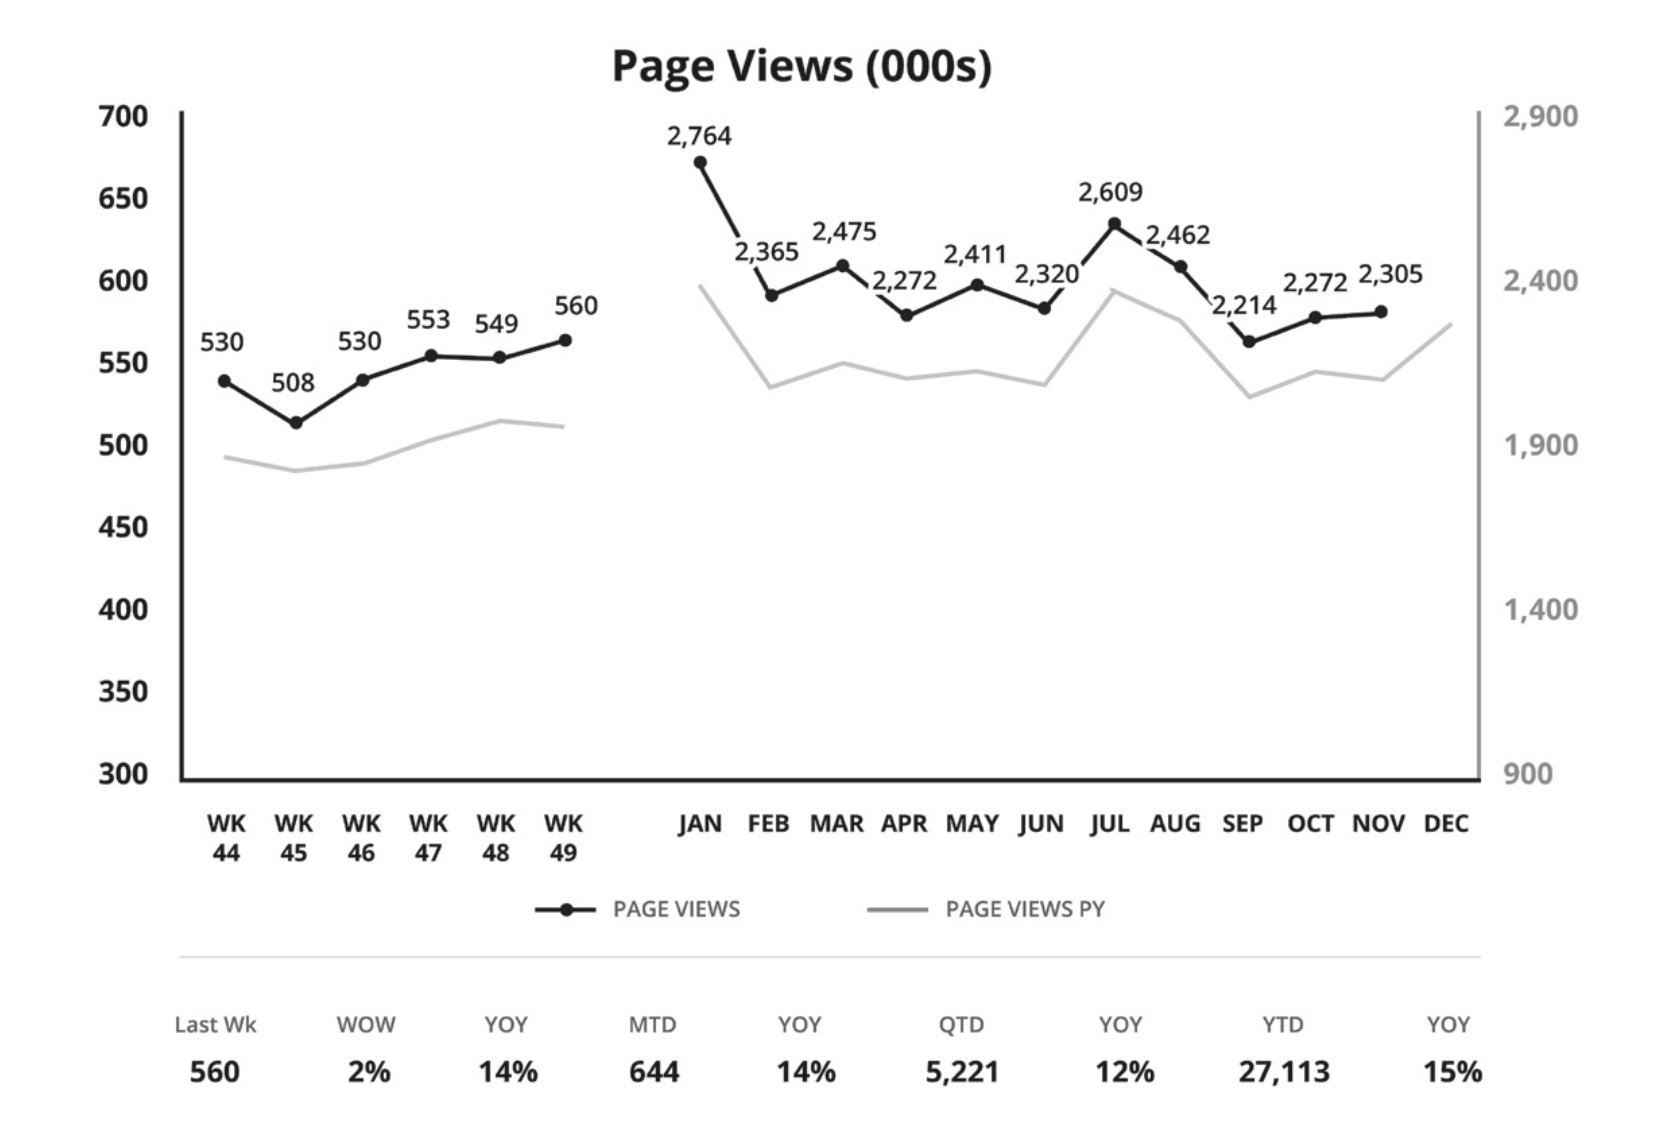
\includegraphics{amazon-page-views-chart.png}
  \end{figure}
  \par This graphic\cite{Bryar2021} measures page views for a business, and conveys a lot of data in a small space:
  \begin{itemize}
    \item{The gray line is prior year, the black line is current year}
    \item{The left graph, those first 6 data points, shows the trailing 6 weeks}
    \item{The right graph, with 12 data points, shows the entire trailing year month by month}
    \item{This built-in “zoom” adds clarity by magnifying the most recent data, which the 12-month graph puts into context.}
  \end{itemize}
  At the bottom of the chart, we call out additional key data points, most of which compare one period to another.\par

%\noindent\makebox[\linewidth]{\rule{\paperwidth}{0.4pt}}

\newpage
\bibliography{MyReport-AzureQuantumElements-MicroGravity}
\bibliographystyle{plainnat}

\end{document}